\section{QuickCheck}
QuickCheck został stworzony w języku Haskell jako pierwsze narzędzie wspierające testowanie oparte na właściwościach. Jest on inspiracją dla bibliotek w innych językach, takich jak FsCheck dla .NET.

\subsection*{Cechy QuickCheck}
\begin{itemize}
    \item Automatyczne generowanie danych testowych.
    \item Sprawdzanie, czy zdefiniowane właściwości funkcji są spełniane dla wielu losowych przypadków.
    \item W przypadku wykrycia błędu narzędzie redukuje (\textit{shrinking}) dane wejściowe, aby znaleźć minimalny przykład prowadzący do błędu.
\end{itemize}

\begin{figure}[h]
    \centering
    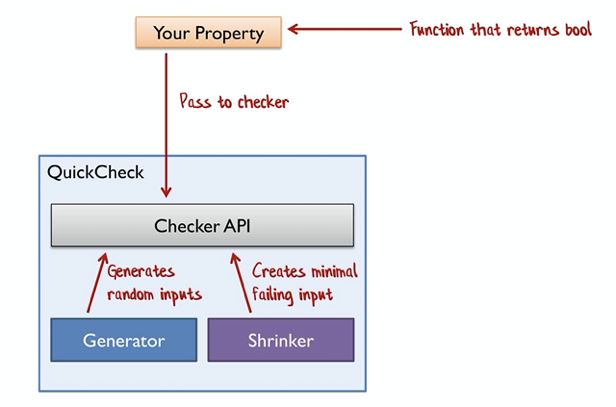
\includegraphics[width=0.8\textwidth]{images/schema.png}
    \caption{Schemat działania QuickCheck}
\end{figure}

\subsection*{Działanie}
\begin{enumerate}
    \item \textbf{Checker API} wykrywa typ wejścia funkcji.
    \item Wywoływany jest generator odpowiedniego typu.
    \item Następuje generowanie przypadków testowych.
    \item Przypadki testowe są przekazywane do testowanej właściwości.
\end{enumerate}

\subsection*{Funkcje}
\begin{itemize}
    \item \textbf{Check.Quick} -- uruchamia szybki test, sprawdzając właściwość dla domyślnej liczby losowych przypadków (np. 100).
    \item \textbf{Check.Verbose} -- działa jak Check.Quick, ale wyświetla więcej szczegółowych informacji o danych testowych.
    \item \textbf{Generowanie danych wejściowych} -- FsCheck wspiera generowanie danych dla typów prostych (np. \texttt{int}, \texttt{float}, \texttt{string}) i bardziej złożonych struktur, takich jak listy czy rekordy.
\end{itemize}

\section*{Pisanie właściwości w FsCheck}

FsCheck umożliwia definiowanie właściwości w formie funkcji logicznych. Właściwości opisują, jakie warunki zawsze muszą być spełnione przez funkcję.

\subsection*{Przykład: Odwracanie listy}
Dla funkcji \texttt{reverse}, która odwraca listę, możemy zdefiniować właściwość:
\begin{itemize}
    \item Odwrócenie listy dwukrotnie powinno zwrócić pierwotną listę.
\end{itemize}

\lstset{language=FSharp, basicstyle=\scriptsize}
\begin{lstlisting}[frame=single,caption={Definicja właściwości dla odwracania listy},label=kod:listingA]
let reverseProperty (xs: int list) =
    List.rev (List.rev xs) = xs

Check.Quick reverseProperty
\end{lstlisting}

\section*{Generacja danych testowych}

FsCheck pozwala na tworzenie własnych generatorów danych wybranego typu. Przydatne, gdy chcemy testować funkcję na specyficznych danych. \\
Na początku tworzymy generator, następnie generujemy dane testowe podając maksymalny rozmiar przypadku testowego (w przypadku stuktur danych) oraz liczbę przypadków testowych.\\
Zarówno przy generowaniu danych testowych, jak i przy późniejszej redukcji danych (shrinking) wykorzystywaniy jest arbitraż (Arb).\\
Jest to mechanizm definiowania sposobu generowania losowych danych dla konkretnego typu. Dzięki arbitrażowi możesz dostosować sposób generowania danych, wprowadzić dodatkowe ograniczenia, a nawet zdefiniować własne typy i ich generatory.

\lstset{language=FSharp, basicstyle=\scriptsize\ttfamily}
\begin{lstlisting}[frame=single,caption={Przykład generatora dla liczb dodatnich},label=kod:listingA]
let intGenerator = Arb.generate<int>
Gen.sample 100 3 intGenerator  // [-37; 24; -62]

// Przyklad generowania liczb dodatnich:
type PositiveInt = PositiveInt of int

let positiveIntGen =
    Gen.suchThat ((<) 0) Arb.generate<int>
Arb.register<PositiveInt>(positiveIntGen)

type Generators =
    static member PositiveInt() =
        Arb.fromGen positiveIntGen
Arb.register<Generators>() // rejestracja generatora by Quick.Check mogl zostac uzyty

let intListGenerator = Arb.generate<int list>
Gen.sample 5 10 intListGenerator 
// [ []; []; [-4]; [0; 3; -1; 2]; [1]; [1]; []; [0; 1; -2]; []; [-1; -2]]

let stringGenerator = Arb.generate<string>
Gen.sample 10 3 stringGenerator // [""; "eiX$a^"; "U%0Ika&r"]

type Point = {x:int; y:int; color: Color}
let pointGenerator = Arb.generate<Point>
Gen.sample 50 10 pointGenerator
(*
{x = -8; y = 12; color = Green -4;};
    {x = 28; y = -31; color = Green -6;};
    {x = 11; y = 27; color = Red;};
    {x = -2; y = -13; color = Red;};
    {x = 6; y = 12; color = Red;};
    // itd
*)
\end{lstlisting}

\section*{Shrinking}

Po fazie generowania danych losowych dane wejściowe są ustawione od najmniejszej do największej wartości. Jeśli jakiekolwiek dane wejściowe spowodują, że właściwość przestanie być spełniona, narzędzie zaczyna "zmniejszać" pierwszy parametr, aby znaleźć mniejszą wartość. Dokładny proces zmniejszania zależy od typu danych (można go również nadpisać) \textit{(W przypadku liczb prowadząc do coraz mniejszych wartości.)}

\lstset{language=FSharp, basicstyle=\scriptsize}
\begin{lstlisting}[frame=single,caption={Przykład shrinking na liczbach},label=kod:listingA]
let isSmallerThan80 x = x < 80
isSmallerThan80 100 // false, so start shrinking

Arb.shrink 100 |> Seq.toList//  [0; 50; 75; 83; 94; 97; 99]
isSmallerThan80 0 // true
isSmallerThan80 50 // true
isSmallerThan80 75 // true
isSmallerThan80 83 // false, so shrink again

Arb.shrink 83 |> Seq.toList//  [0; 44; 66; 77; 80; 81; 83]
isSmallerThan80 0 // true
isSmallerThan80 44 // true
isSmallerThan80 66 // true
isSmallerThan80 77 // true
isSmallerThan80 80 // false <- najmniejsza porazka
// wynik: Falsifiable, after 10 tests (2 shrinks)
\end{lstlisting}

Narzędzie jest bardzo przydatne do określenia, gdzie znajdują się granice błędów w testowaniu\\
Shrink działa na customowych typach złożonych, dodatkowo można też generować własne sekwencje oraz zasady w jaki sposób przeprowadzać customowe shrinkowanie. 

\lstset{language=FSharp, basicstyle=\scriptsize}
\begin{lstlisting}[frame=single,caption={Shrinkowanie ciągu znaków},label=kod:listingA]
Arb.shrink "abcd" |> Seq.toList
// ["bcd"; "acd"; "abd"; "abc"; "abca"; "abcb"; "abcc"; "abad"]
\end{lstlisting}

\section*{Konfiguracja}
Czasem może zaistnieć potrzeba własnego dostosowania liczby testów itp. W tym celu można odpowiednio skonfigurować narzędzie:
\lstset{language=FSharp, basicstyle=\scriptsize}
\begin{lstlisting}[frame=single,caption={Dostosowanie konfiguracji testów},label=kod:listingA]
let config = {
    Config.Quick with
        MaxTest = 1000
    }
    Check.One(config,isSmallerThan80 )
    // result: Ok, passed 1000 tests. (a nie powinno :)
    
    let config = {
    Config.Quick with
        MaxTest = 10000
    }
    Check.One(config,isSmallerThan80 )
    // result: Falsifiable, after 8660 tests (1 shrink):
    //         80
\end{lstlisting}

\section*{Warunki wstępne}
\lstset{language=FSharp, basicstyle=\scriptsize}
\begin{lstlisting}[frame=single,caption={Dodawanie warunków wstępnych},label=kod:listingA]
let preCondition x y =
    (x,y) <> (0,0)
    && (x,y) <> (2,2)

let additionIsNotMultiplication_withPreCondition x y =
preCondition x y ==> additionIsNotMultiplication x y
// Ok, passed 100 tests.
\end{lstlisting}

Jak widać, tego rodzaju rozwiązania mogą być użyte tylko w nielicznych przypadkach, gdy możemy zdefiniować niewielką liczbę "wyjątków od reguły".

\section*{Testowanie kilku właściwości na raz}
W celu zapewnienia uporządkowania i ustrukturyzowania kodu istnieje możliwość testowania kilku włąsciwosci równocześnie.
\lstset{language=FSharp, basicstyle=\scriptsize}
\begin{lstlisting}[frame=single,caption={Sprawdzanie wielu właściwości jednocześnie},label=kod:listingA]
type AdditionSpecification =
    static member ``Commutative`` x y =
      commutativeProperty x y
    static member ``Associative`` x y z =
      associativeProperty x y z
    static member ``Left Identity`` x =
      leftIdentityProperty x
    static member ``Right Identity`` x =
      rightIdentityProperty x
  
Check.QuickAll<AdditionSpecification>()

--- Checking AdditionSpecification ---
AdditionSpecification.Commutative-Ok, passed 100 tests.
AdditionSpecification.Associative-Ok, passed 100 tests.
AdditionSpecification.Left Identity-Ok, passed 100 tests.
AdditionSpecification.Right Identity-Ok, passed 100 tests.
\end{lstlisting}